\documentclass[journal]{IEEEtran}
% IEEE Transactions on Industrial Informatics -- anonymous regular-paper draft
% Compile: latexmk -pdf main.tex
\usepackage{amsmath,amssymb,amsfonts}
\usepackage{algpseudocode}
% Local XeTeX/Tectonic builds: route IEEEtran's ptm (Times) family requests to
% the legacy Times Type1 faces so metrics match the pdfLaTeX reference build;
% the latexmk -pdf (pdfLaTeX) path is unaffected.
\usepackage{iftex}
\ifxetex
  \DeclareFontFamily{TU}{ptm}{}
  \DeclareFontShape{TU}{ptm}{m}{n}{<->ptmr8t}{}
  \DeclareFontShape{TU}{ptm}{b}{n}{<->ptmb8t}{}
  \DeclareFontShape{TU}{ptm}{m}{it}{<->ptmri8t}{}
  \DeclareFontShape{TU}{ptm}{b}{it}{<->ptmbi8t}{}
  \DeclareFontShape{TU}{ptm}{m}{sl}{<->ptmro8t}{}
  \DeclareFontShape{TU}{ptm}{m}{sc}{<->ptmr8t}{}
\fi
\usepackage{graphicx}
\usepackage{booktabs}
\usepackage{tabularx}
\usepackage{array}
\usepackage[table]{xcolor}
\usepackage{stfloats}
\usepackage{placeins}
\usepackage{url}
\usepackage{etoolbox}
\usepackage{balance}
\urlstyle{same}
% Cross-references and citations. The cite package renders IEEE-style citation
% groups ([14]--[16], [20], [21]) with hyperref support.
\usepackage{cite}
\usepackage[colorlinks=true,linkcolor=black,citecolor=black,urlcolor=black]{hyperref}
\hypersetup{bookmarksnumbered=true,
  pdftitle={Configuration-Driven Integration of Industrial Agents Across Production Scenes},
  pdfauthor={},
  pdfsubject={IEEE Transactions on Industrial Informatics},
  pdfkeywords={industrial agents, industrial communication, industrial informatics, production systems, semantic data integration}}

% Float placement only; IEEEtran margins and body type remain unchanged.
\setcounter{topnumber}{4}
\setcounter{bottomnumber}{3}
\setcounter{totalnumber}{7}
\setcounter{dbltopnumber}{2}
\renewcommand{\topfraction}{0.95}
\renewcommand{\bottomfraction}{0.80}
\renewcommand{\textfraction}{0.03}
\renewcommand{\floatpagefraction}{0.72}
\renewcommand{\dbltopfraction}{0.95}
\renewcommand{\dblfloatpagefraction}{0.72}

% Tight but conventional float separation; body type and margins are unchanged.
\setlength{\textfloatsep}{8pt plus 2pt minus 3pt}
\setlength{\dbltextfloatsep}{8pt plus 2pt minus 3pt}
\setlength{\intextsep}{7pt plus 2pt minus 3pt}
\setlength{\abovecaptionskip}{3pt plus 1pt minus 1pt}
\setlength{\belowcaptionskip}{2pt plus 1pt minus 1pt}

\newcommand{\system}{the platform}
% Review copy is anonymous. The AI-use statement is maintained in
% AI-DISCLOSURE.md for the journal-approved disclosure channel and is not
% compiled into this manuscript.
\newif\ifblindreview
\blindreviewtrue

\begin{document}
\bstctlcite{IEEEbstctl}

\title{Configuration-Driven Integration of Industrial Agents Across Production Scenes}

\author{}
\markboth{IEEE Transactions on Industrial Informatics, Submitted Manuscript}{Industrial Agent Integration}

\maketitle

\begin{abstract}
Industrial production scenes vary in process context, signal semantics, and
communication protocols, while task-level agents require bounded access to
equipment operations. A deployment must therefore connect scene-specific
context and I/O mappings to a common task-operation interface and check each
write against current authority and configured limits. This paper presents a
configuration-driven architecture that binds line--product--recipe--run
context and semantic data-acquisition and write-control nodes to protocol
drivers and named operations. Harness adapters separate agent-turn execution
from scene-specific I/O, and a shared dispatcher applies authority and
route-specific write checks.

We evaluated one integrated deterministic-simulator run. The primary
cast-film configuration returned 54 acquisition samples, and all 24 negative
probes across four writable paths were rejected by write-admission checks. A
second configuration, tested within the same run, returned 51 samples and
rejected all nine probes across three writable paths. The run passed 76 of 77
checks, with one warning and no failed checks. Three fixed-seed objective
cases had end scores at 96.3\%--98.8\% of the simulator's offline reference;
one case stopped before any update. These results show that selected scene
mappings, protocol routes, and guards operated together in the tested
simulator. The language-model loop and physical equipment were not used; the
results therefore do not establish real-harness interchangeability,
autonomous-agent performance, comparative control benefit, repeatability, or
field operation.
\end{abstract}

\begin{IEEEkeywords}
Industrial agents, industrial communication, industrial informatics,
production systems, system integration.
\end{IEEEkeywords}

\IEEEpeerreviewmaketitle

\section{Introduction}
\IEEEPARstart{I}{ndustrial} production systems expose measurements and control
points through interfaces that vary by process line, device, and communication
protocol. A task-level agent therefore needs more than a list of tools: it must
receive the active line, product, recipe, and run context, address the intended
control node, and operate within the limits configured for that process. A
command receipt also has a different meaning from a subsequent process
measurement. In the cast-film simulator used in this study, for example, line
speed is configured through a message-queuing protocol while film thickness is
acquired as a process value. In the evaluated scene, the MQTT endpoint carries
the line-speed setpoint and returns thickness samples; this configured pairing
does not by itself establish that a write caused a measured change. The
architecture must preserve the relation between those signals without treating
a successful write as proof of a desired process response.

Research on industrial agents addresses process supervision, control
generation, service selection, and human-guided automation
\cite{xia2025control,huang2026made,koehle2026llmdriven,biskupovic2025supervision,
liu2026agents4plc,wu2025instructmpc,lim2025llmenabled,zhao2026shopfloor,
hofmann2025nlc}. Other work connects agents with digital twins, manufacturing
skills, and shop-floor services
\cite{xia2025architecture,silva2025mcpmanufacturing,
koehle2025semanticrecipes,graul2026aas,schall2026safe,lin2026agentic}.
Industrial-informatics architectures have also formalized trust boundaries for
digital-twin control, functional blocks for industrial IoT networks, and
security services at the fog layer
\cite{gehrmann2020dtiacs,mahmood2023functional,sengupta2021securefog}.
Together, these studies provide methods for agent reasoning, asset grounding,
communication, and secure service execution. They motivate a complementary
deployment question: how should a system bind different production scenes and
agent runtimes to the same governed operation boundary?

This work addresses that integration boundary. It designs and implements a
configuration-driven architecture in which production context and
protocol-specific I/O are defined by scene configuration, while harness
adapters present agent engines through a common task-operation interface.
Task-mediated calls and direct operation calls converge on shared dispatch
checks, and each device write is evaluated against the live context and the
limits configured for its route. The contribution is a system architecture
and its implementation, rather than a new control law or an autonomous-agent
algorithm.

The paper makes two architectural contributions:
\begin{enumerate}
  \item A scene configuration binds line--product--recipe--run context to
  semantic data-acquisition and write-control nodes, protocol drivers,
  objectives, and engineering limits. The mappings remain explicit per scene
  behind a common operation interface.
  \item A task-to-device runtime separates harness turn execution from
  scene-specific I/O. Task calls and direct operation calls enter a shared
  dispatcher, which checks authority and current context before route-specific
  limits and any required approval are applied. Service-owned records keep
  command receipts distinct from later process observations.
\end{enumerate}

The evaluation tests selected links across this architecture in a deterministic
simulator execution. Its scope and evidence limits are stated with the results;
the run does not establish real-harness interchangeability or field operation.

Section~II positions the integration problem among industrial-agent and
industrial-informatics architectures. Section~III describes the system
architecture and execution contract, and Section~IV details context assembly,
write admission, approval revalidation, and record semantics. Section~V
reports distinct evidence blocks from the single simulator execution:
workflow coverage, protocol acquisition and guard checks, seeded objective
cases, and a separately scripted BOPET integration trace. Sections~VI and
VII discuss what these observations support and where the evidence ends.

Fig.~\ref{fig:control-path} summarizes how scene-bound context and I/O mappings
meet the shared dispatch boundary before a configured driver is invoked.

\begin{figure}[!b]
\centering
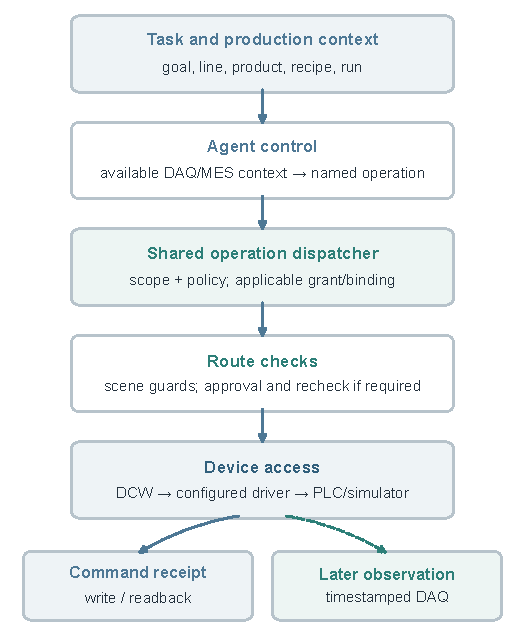
\includegraphics[width=\columnwidth]{resources/fig1-nature-A.pdf}
\caption{Task execution from process context to device observation. Data
acquisition (DAQ) and manufacturing execution system (MES) services provide
process context for a named operation. Shared
dispatch checks precede route-specific limits and any required approval and
context revalidation. Configured drivers access the device; the command
receipt and later process measurement remain separate records.}
\label{fig:control-path}
\end{figure}

\section{Related Work}
\label{sec:related}
Table~\ref{tab:nearest} summarizes selected studies that connect agents or
software services to industrial equipment, production data, or process
operations. The studies locate the integration problem addressed here; they
are not matched performance baselines.

\subsection{Industrial Agents and Plant Integration}
Industrial-agent studies span process supervision, control generation, and
equipment-facing assistance. Large language model (LLM) frameworks address
end-to-end automation and industrial cyber-physical-system control
\cite{xia2025control,huang2026made}; related work generates programmable
logic controller (PLC) code or
combines human guidance with control
\cite{liu2026agents4plc,wu2025instructmpc}. Other studies examine resource
capabilities, shop-floor coordination, and digital-twin fault handling
\cite{lim2025llmenabled,zhao2026shopfloor,gill2025llmdt}, as well as
natural-language machine access and robotic-line control
\cite{hofmann2025nlc,waseem2026pretrained}. Biskupovic et al. are especially
close in using agents to supervise industrial systems: their agents select
services from a component library using performance and computational-load
metrics, monitor online performance, and reconfigure service selection when
performance degrades \cite{biskupovic2025supervision}. Taken together, this
strand studies agent behavior at the level of control, service choice, or
equipment interaction; the question here is how those agents connect to
scene-specific signals and governed operations.

Xia et al. connect cognitive, digital-twin, and physical-automation layers and
organize twin information as state snapshots, event messages, and plan
sequences \cite{xia2025architecture}. Other nearby designs expose factory-module
operations through the Model Context Protocol (MCP) with state-based tool
filtering, constrain manufacturing plans, or compose semantic recipes from
OPC Unified Architecture (OPC UA) skills
\cite{koehle2026llmdriven,silva2025mcpmanufacturing,koehle2025semanticrecipes}.
Several recent systems also combine agent execution with approval, industrial
data, or audit records. Graul et al. ground proposals in the Asset
Administration Shell (AAS) and route approved actions through OPC UA Methods,
with signed approvals and audit logging \cite{graul2026aas}. Schall separates
advisory language-model agents from process and instrumentation diagram
(P\&ID)-grounded verification and execution, and evaluates structural checks
across five simulated process scenarios \cite{schall2026safe}; its context
includes supervisory control and data acquisition (SCADA) and standard
operating procedure (SOP) information. Lin and Chen build a governed digital
thread across sensors, the manufacturing execution system (MES), and enterprise
resource planning (ERP) for closed-loop monitoring and control on real
manufacturing records \cite{lin2026agentic}. These systems address
complementary parts of industrial-agent deployment, including process
reasoning, service adaptation, asset grounding, action validation, and
evidence organization. This paper addresses a related but distinct integration
boundary: how to connect replaceable agent harnesses and task roles to
different configured production scenes while preserving
line--product--recipe--run context, semantic signal mappings, and a governed
parameter-write path. Whereas Biskupovic et al. study agent-based service
selection and reconfiguration, this architecture centers on scene configuration
and a shared operation boundary that resolves configured device nodes and
retains command receipts separately from process observations. The contribution
is an integration architecture and implementation, not a new process-control
law. Table~\ref{tab:nearest} compares reported mechanisms and evaluation
settings only; it does not rank features or performance.
\begin{table*}[!t]
\centering
\caption{Reported operation mechanisms and evaluations in selected
plant-facing studies. Evaluation settings and outcomes are source-specific;
this table does not compare performance across studies.}
\label{tab:nearest}
\small
\setlength{\tabcolsep}{3pt}
\begin{tabularx}{\textwidth}{@{}>{\raggedright\arraybackslash}p{1.8cm}>{\raggedright\arraybackslash}p{7.0cm}>{\raggedright\arraybackslash}X@{}}
\toprule
System & Reported operation or integration mechanism & Reported evaluation \\
\midrule
Xia et al. \cite{xia2025architecture} & Cognitive, twin, and physical layers; twin snapshots, event messages, and plan sequences & Robotic automation and process-simulation cases \\
Biskupovic et al. \cite{biskupovic2025supervision} & Agent-based selection and online reselection of services using performance and computational-load metrics & Reported adaptability and performance improvement in service-oriented industrial cyber-physical systems \\
K{\"o}hle et al. \cite{koehle2026llmdriven} & Injected live state and state-based filtering; MCP-to-OPC UA operations and Message Queuing Telemetry Transport (MQTT) coordination & Nine simulated production challenges \\
Vieira da Silva et al. \cite{silva2025mcpmanufacturing} & Constrained multi-step plans over MCP manufacturing functions & Laboratory multi-step process \\
K{\"o}hle et al. \cite{koehle2025semanticrecipes} & Semantic recipes composed from OPC UA skills; virtual commissioning & Unity assembly-workstation proof of concept \\
Graul et al. \cite{graul2026aas} & AAS-grounded proposals, signed human approval, PLC-validated OPC UA Methods, and immutable audit log & Two laboratory PoCs; single scripted runs \\
Lin and Chen \cite{lin2026agentic} & Governed sensor--MES--ERP digital thread with SOP-, risk-, and capability-aware action gating & 25,275 real records; operational metrics \\
Schall \cite{schall2026safe} & P\&ID-, SCADA-, and SOP-grounded proposal verification with gated execution & Five simulated scenarios; 43 proposals and 50 LLM runs \\
\midrule
This work & Common task-operation interface with registered harness adapters; scene-bound context and acquisition/write-node mappings; bounded named operations; separate command and observation records & One deterministic integrated simulator run; distinct protocol and guard checks, fixed-seed objective cases, and a scripted BOPET integration trace \\
\bottomrule
\end{tabularx}
\end{table*}

Industrial-informatics architectures offer complementary design precedents.
Gehrmann and Gunnarsson define trust boundaries and synchronization
requirements for digital-twin-based industrial control and evaluate a
protected-update proof of concept
\cite{gehrmann2020dtiacs}. Mahmood et al. organize special-purpose industrial
IoT functions around network requirements, while Sengupta et al. distribute
security services across fog and device layers and report simulation and
testbed evidence \cite{mahmood2023functional,sengupta2021securefog}. These
works address communication, security, and functional decomposition. The
present system focuses on a different interface: binding scene-specific
context and device mappings to task-level operations while retaining
execution-time checks and separate command and process records. Its operation
checks complement safety-aware decision support
\cite{jiang2026agentic} and do not replace configured plant protection.

\subsection{Production Context, Agent Interfaces, and Automation}
Industrial integration also depends on abstractions that are not specific to
agent architectures. The Model Context Protocol (MCP) specifies interoperable
tool discovery and call mechanisms \cite{mcp2024}. The platform dispatcher's
operation-level scope, policy, grant, and binding checks are distinct from MCP
transport authorization. In parallel,
ISA-88 and ISA-95 describe recipes and production operations
\cite{isa88_2010,isa95_2025}. Run-to-run methods connect process observations
to successive production runs \cite{moyne2000r2r}. Human--automation research
also formalizes the allocation of information acquisition, analysis, decisions,
and actions between people and automation \cite{parasuraman2000model}. At the
agent level, AgentSpec and CaMeL address tool behavior and capability-based
information flow \cite{wang2025agentspec,debenedetti2025camel}. These
standards and concepts inform the design's treatment of production context,
tool interaction, human allocation, and information-flow boundaries; their
mention does not imply implementation of every listed standard or safety
mechanism. Within this selected literature, these concerns are treated through
separate interfaces and validation layers; how to bind scene context and
heterogeneous I/O to a shared task-operation interface and write-governance
path remains under-specified. This paper addresses that integration question,
and the evaluation tests selected links in a deterministic simulator run.

\section{System Design}
\label{sec:design}
The architecture connects two configurable sides of an industrial deployment:
an agent collaboration runtime and a production-scene configuration. The
runtime supplies task context and scoped operations; scene configuration maps
process semantics to acquisition and control nodes, drivers, targets, and
guards. Named operations connect these sides to shared dispatch and governed
device access. The design separates task execution from operation dispatch and
keeps command receipts distinct from measured process responses.

\begin{figure*}[!t]
\centering
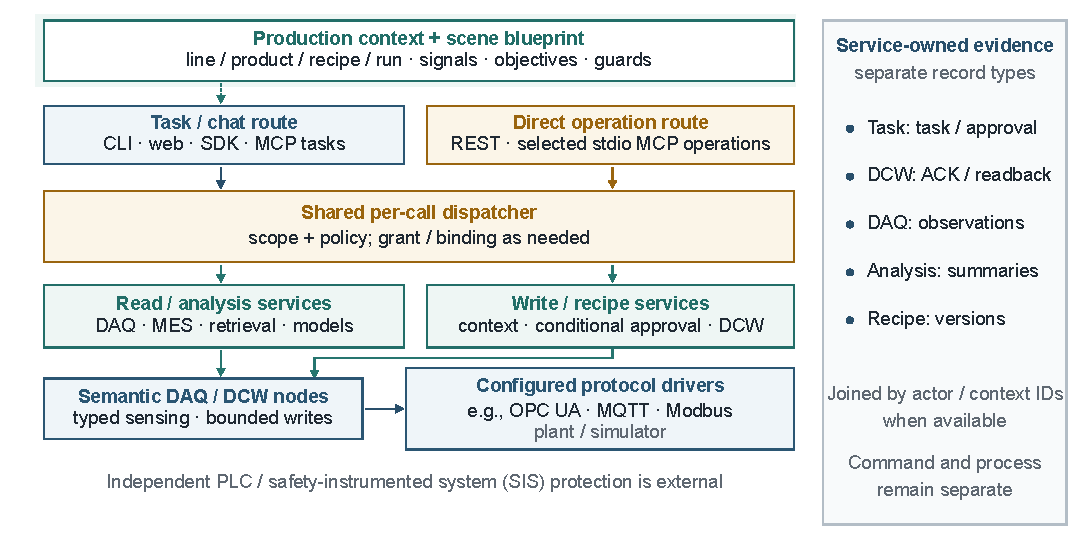
\includegraphics[width=\textwidth]{resources/fig-architecture-2026-9pt.pdf}
\caption{Architecture and record ownership. Task/chat routes enter the
collaboration runtime; direct REST and stdio-MCP calls enter shared dispatch
checks without creating a task. One dashed link marks configuration. Write
routes apply interval admission and, when configured, approval; recipe dispatch omits the
previous-recipe window. The shared dispatcher always
checks scope and channel policy, with grant and resource-binding checks applied
when required by the operation. Owning services retain distinct records; plant
controllers and safety systems retain equipment interlocks.}
\label{fig:arch}
\end{figure*}

\subsection{Design Rationale and Requirements}
\label{sec:principles}
Three design requirements follow from the deployment problem. Scene
configuration must preserve process meaning while mapping signals and controls
to heterogeneous drivers. Harness variation must not change the operation
contract. Each write must also be checked against current authority and
process limits, with its command receipt distinguishable from later process
measurements. The architecture addresses these requirements through
scene-bound data-acquisition and write-control nodes, registered harness
adapters, a shared dispatcher, and service-owned records. The registry
provides an extension point for additional agent engines and protocol drivers;
the experiment evaluates only the configured simulator paths described in
Section~\ref{sec:eval}. Tool visibility alone does not authorize a write:
actuator operations pass through the shared write-admission point.

Commissioning associates the line with products, recipes, active-run rules,
signal meanings, units, driver mappings, and admissible limits. At runtime,
the context builder assembles the active line--product--recipe--run state and
relevant process summaries for each agent turn. An operation handler resolves
live state again before dispatch, so the prompt context informs a proposal but
does not substitute for current authorization or admission checks. Direct
operations resolve the current context at invocation without creating a task.

\subsection{Layered Architecture}
\label{sec:layers}
\label{sec:arch}
Fig.~\ref{fig:arch} summarizes the access routes, shared dispatch path,
production services, semantic I/O, configured drivers, and service ownership
of records. Task and chat routes enter the collaboration runtime, which
contains workspaces, channels, task queues, shared memory, mailboxes, task
templates, and harness adapters. A \emph{task route} is an execution path
through this runtime; a \emph{harness adapter} connects an agent engine to its
task interface. Multiple registered agents can participate through shared
tasks and channel context, with each agent's available tools constrained by
its binding and channel policy. Direct REST tool
calls and the stdio MCP operation bridge bypass task execution in that band
(the upper-right direct-operation entry in
Fig.~\ref{fig:arch}) and enter the shared governance block without creating a
task or starting a harness turn; MCP management and task methods remain on
their service routes. Direct calls resolve current route state at invocation,
without an agent-turn prompt or a task record.
The governance block projects the operation catalog and applies the per-call
checks. Write handlers apply admission limits and request approval when the
operation and its configuration require it. The
context block supplies the active line--product--recipe--run tuple to the gate
and scene maps, objectives, and guards to the handlers. The dashed link from
that block in Fig.~\ref{fig:arch} marks this configuration relationship; the
runtime assembles prompt-time context from the same records. The service band,
behind a route-handler interface that selects an adapter, provides data
acquisition, write control, analysis, retrieval, and optional model services.
Field I/O resolves semantic nodes to built-in or plugin drivers for a plant or
simulator. Services retain task, command, observation, and configuration
records separately and associate them with actor and production context.

\subsection{Cross-Module Execution Flow}
\label{sec:executionflow}
Fig.~\ref{fig:runtime} summarizes a task turn from entry through operation
execution, with route-specific evidence retained by owning services. Registered
harness adapters receive a scoped tool catalog during setup and supported
registry refreshes; the runtime assembles prompt-time production context from
current records for each agent turn. For each returned tool call, the shared
dispatcher rechecks invocation scope, channel policy, and applicable grant and
binding conditions before handler selection. The selected handler
then applies route-specific guards, active-run checks, approval
revalidation, and device-I/O steps as applicable. Command receipts and later
process observations remain distinct records.

For an industrial operation $u$ by agent $a$ in channel $c$, define the
shared dispatch condition as
\begin{equation}
\mathcal{A}(a,c,u)=\bigwedge_{X\in\mathcal{C}(u)}X(a,c,u),
\label{eq:dispatch-contract}
\end{equation}
where $S$, $P$, $G$, and $B$ denote invocation scope, current channel policy,
applicable industrial grant, and the agent's binding to referenced resources,
respectively. $\mathcal{C}(u)\subseteq\{S,P,G,B\}$ is the set of predicates
declared for operation $u$; it always contains $S$ and $P$. The grant predicate
$G$ is included when the resolved channel, target line, and owner/grant policy
require it; explicit exemptions omit it. The binding predicate $B$ is included
when the operation declares resource references. A declared no-reference
operation omits $B$. Each included check must pass before
handler selection. The policy predicate includes channel tool selection,
profile, and duty-separation checks where configured. Once these predicates
pass, the selected route applies its guards, active-run checks, admission
limits, and any required approval. When approval is required, the handler
revalidates its context before device dispatch.

For direct REST invocation, the service establishes $a$ and $c$ before applying
these checks: an agent token must match the requested agent identifier, or an
authenticated user must be the channel owner or an administrator. The manager
loads the channel-agent record and rechecks scope and policy; applicable grant
and binding checks follow. Handlers resolve live
production state from request identifiers and owning services.

Fig.~\ref{fig:execution} gives reference pseudocode summarizing the
registered-harness task path. Direct REST tool invocation
bypasses the task runtime and harness but enters the same shared dispatcher.
Route-specific timing, approval, and evidence rules are detailed in
Section~\ref{sec:modules}.

\begin{figure*}[!t]
\centering
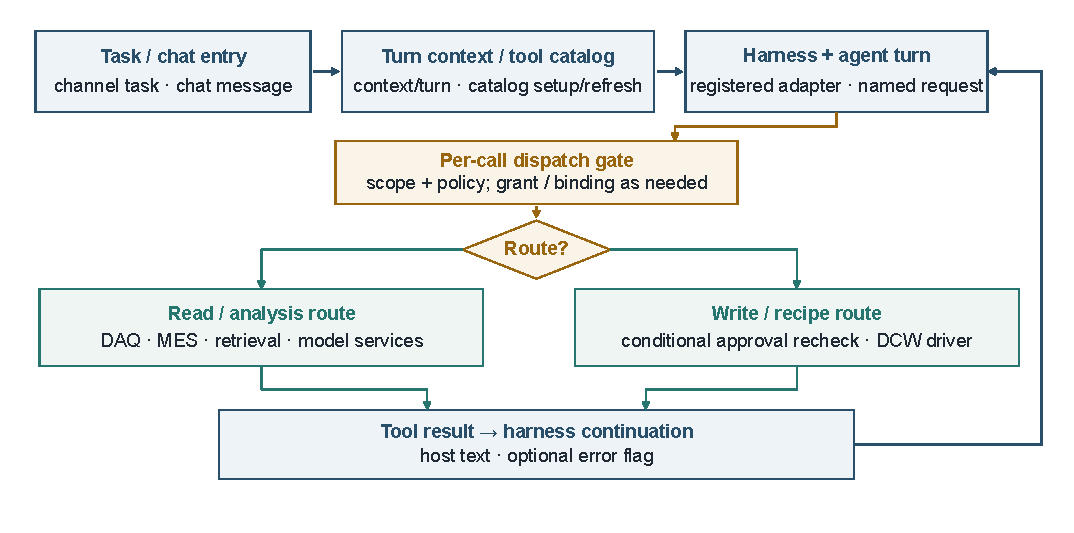
\includegraphics[width=\textwidth]{resources/fig-runtime-2026-9pt.pdf}
\caption{Registered-harness task flow. The runtime invokes the adapter with a
scoped catalog. Scope and channel policy are checked for every call; grant
applies to non-exempt industrial operations, and binding applies when resource
references are declared. Failed checks return tool errors. The read path
retrieves data. The write path applies route guards, conditional approval and
its context revalidation, write admission, and receipt grading; a later process
observation is separate. Results return to the harness. Device-level interlocks remain
with the configured plant-control layer.}
\label{fig:runtime}
\end{figure*}

\begin{figure}[!t]
\centering
\begin{algorithmic}[1]
\Require task $q$, channel $c$, bound agent $a$, registered scoped catalog $T$
\Ensure task result; any retained evidence remains with its owning service
\State $x_t \gets \Call{ResolvePromptContext}{c,q}$
\State $m \gets \Call{RetrieveMemory}{q}$
\State $p \gets \Call{AssemblePrompt}{q,x_t,m}$
\State $h \gets \Call{InvokeRegisteredHarness}{a,p,T}$
\ForAll{tool request $u$ returned by $h$}
  \State $g \gets \Call{CheckScopeAndChannelPolicy}{a,c,u}$
  \If{\textbf{not} $g$}
    \State \Call{EmitToolErrorToHarness}{h,u}; \textbf{continue}
  \EndIf
  \If{$u$ is an industrial operation}
    \State $v \gets \Call{CheckApplicableGrantBinding}{a,u}$
    \If{\textbf{not} $v$}
      \State \Call{EmitToolErrorToHarness}{h,u}
      \State \textbf{continue}
    \EndIf
  \EndIf
  \State $k \gets \Call{SelectHandler}{u}$
  \State $r \gets \Call{ExecuteRouteHandler}{k,a,c,u}$
  \Comment{handler resolves live state and may persist route-specific records}
  \State \Call{EmitDeclaredToolResultToHarness}{h,r}
\EndFor
\State \Return task state and tool results
\end{algorithmic}
\caption{Reference pseudocode for the registered-harness task path. Direct
operation calls use the shared dispatcher from their own entry point. Each
route persists records through its owning service and returns its declared
response to its caller; task-route results return to the harness.}
\label{fig:execution}
\end{figure}

\section{Module Functions and Integration}
\label{sec:modules}
Section~\ref{sec:design} defines the architecture and shared dispatch
contract. This section specifies the runtime context passed to adapters and
the route-specific admission, approval, and evidence steps.

\subsection{Task, Harness, and Context}
Task and chat entry points create or join a workspace channel. The task
runtime manages membership, roles, task state, and shared execution context;
a harness registry adapts agent engines to a common execution interface. This
separation lets agents collaborate through shared tasks and channel resources
without coupling their engine-specific turn protocol to a production scene.
At each turn, the prompt builder assembles the task, active scene description,
line--product--recipe--run state, channel profile, agent binding, and retrieved
memory. The resulting context supports process-aware proposals, while the
dispatcher independently checks authority and the operation handler resolves
current state before a write.

Direct REST and selected stdio-MCP operation calls reach the same dispatcher
without a task or harness turn. REST authentication and identity resolution
follow Section~\ref{sec:executionflow}; each handler reads live route state
at invocation. Handlers receive the resolved actor, channel, and operation
arguments through the same interface for either entry route; records are keyed
by the identifiers supplied in each request. A registered task additionally
receives prompt context and a scoped tool catalog. Catalog visibility alone
does not grant write authority: the dispatcher checks authority at invocation.

\subsection{Shared Dispatch and Device Admission}
\label{sec:governed}
Each operation must satisfy the predicates in
Eq.~(\ref{eq:dispatch-contract}) before handler selection; the selected
handler then revalidates route-specific state. Scene configuration maps
semantic signals and controls to
drivers and specifies process objectives and guards. Capability profiles and
tool policies narrow available operations, while resource bindings constrain
accessible nodes, controls, and recipes. Optional data-acquisition (DAQ),
manufacturing execution system (MES), analysis, retrieval, optimization, and
digital-twin services are invoked through registered handlers. The application supplies its optimization strategy;
the framework coordinates context, operation access, and execution.

The target band describes a desired process outcome. It is not the admissible
write interval: the latter is computed from engineering, product, recipe, and
route-specific limits below. A candidate can satisfy every write constraint
while the measured process value remains outside its target band.

Actuator writes converge on the shared device-write admission point.
For an online node write, the admissible value interval is
\begin{equation}
\mathcal{I}^{\mathrm{online}}_n(t)=
\mathcal{H}_n\cap\mathcal{L}^{\mathrm{base}}_n\cap\mathcal{L}^{\mathrm{prod}}_n(t)\cap\mathcal{L}^{\mathrm{rec}}_n(t),
\label{eq:admission}
\end{equation}
where $\mathcal{H}_n$ is the hard engineering range and
$\mathcal{L}^{\mathrm{base}}_n$, $\mathcal{L}^{\mathrm{prod}}_n$, and
$\mathcal{L}^{\mathrm{rec}}_n$ are the baseline, active-product, and
active-recipe limits; the $\mathcal{L}$ limits here are deliberately named
apart from the policy and binding predicates of
(\ref{eq:dispatch-contract}). Missing optional limits impose no
restriction; an empty intersection rejects the request and identifies the
excluding layer. Recipe dispatch validates the replacement recipe against
the hard, baseline, and product limits rather than the previous recipe
window. Step, interval, and hold-window checks apply as configured for each route.
These application-level checks bound commands alongside independent
programmable-logic-controller and safety-instrumented protection. They do not
replace equipment interlocks or certify the safety of a plant deployment.

\subsection{Approval, Execution, and Evidence}
\label{sec:routes}
\label{sec:mech}
\label{sec:objective}
\label{sec:nodeexec}
\label{sec:ack}
\label{sec:agentloop}
Routes add timing checks and, when required by operation and configuration,
approval checks. Outside benchmark mode, online agent and manual node writes
enforce a 60\,s minimum interval between successful writes. Recipe trials use
a per-line cadence (300\,s by default), and recipe intervals are anchored to approval.
Manual approval binds an actor and proposed operation to candidate values,
applicable limits, expiry, and the active line--product--recipe--run tuple.
After approval, the handler rechecks authority and compares the current tuple
with the approved tuple before entering device-write dispatch. Single-parameter waits
expire after 180\,s by default; recipe-dispatch approvals use a 30-minute
window. A changed recipe definition requires a new
\texttt{recipe\_apply} proposal.

Fig.~\ref{fig:hitl}(a) illustrates the four-layer interval in
Eq.~(\ref{eq:admission}) as a conceptual intersection of configured bounds;
its horizontal positions do not represent measured or run-derived values.
Panel (b) shows the decision and rechecks when approval is required.

\begin{figure*}[!t]
\centering
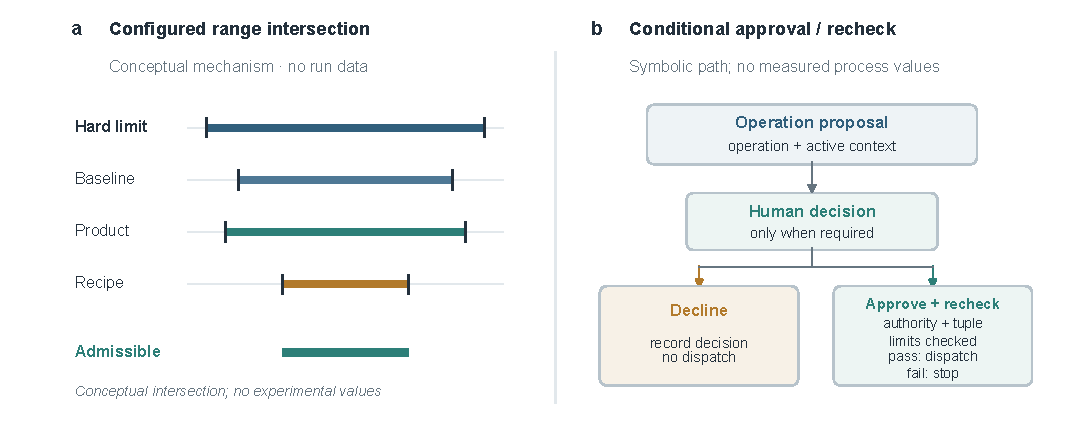
\includegraphics[width=\textwidth]{resources/fig5-nature-A.pdf}
\caption{Admission and approval boundaries. (a) Conceptual intersection of
the hard, baseline, product, and recipe bounds in Eq.~(\ref{eq:admission});
horizontal positions are schematic and encode no experimental values.
(b) When approval is required, a decline prevents dispatch; approval is
followed by authority, context, and limit rechecks.}
\label{fig:hitl}
\end{figure*}

A \texttt{recipe\_trial} illustrates the operation sequence: the handler
checks the bound recipe, active run, candidate parameters, and route timing;
if required, it requests approval; after revalidation, it submits a bounded
batch through the configured driver and returns a per-parameter receipt.
The caller can obtain later DAQ observations separately and may then update,
apply, or roll back a recipe. A trial neither saves nor applies a recipe
version. The driver registry maps semantic controls to configured protocol
drivers, keeping protocol details out of agent operation arguments.

At dispatch, the handler resolves the active production context, intersects
the applicable bounds, and applies route timing and approval requirements
before invoking the configured driver. The driver returns a graded receipt;
later acquisition samples are stored separately and linked to the operation
when the route provides matching context and timestamps. The evaluation uses
deterministic tool invocation and does not assess operator performance.

Receipts and observations answer different questions. A command result is
graded as readback-verified, transport-acknowledged, or unverified; a
readback mismatch can trigger up to three reads at 2\,s intervals. Recipe
batches retain per-parameter verification outcomes. A readback-verified result
records that the returned value matched the request; a transport acknowledgement
alone does not establish that the device applied it, and an unverified result
does not establish a matching readback. DAQ stores subsequent timestamped
process observations, while recipe history, approvals, and task records remain
with their owning services. Identifiers and timestamps can link these records
when available, but a later observation alone does not prove that the command
caused the measured change. Section~\ref{sec:eval} evaluates selected parts of
this evidence chain under the stated test conditions.


\section{Experimental Evaluation}
\label{sec:eval}
This evaluation reports one integrated pipeline execution. It contains
separate evidence blocks for workflow coverage, protocol acquisition and
write guards, fixed-seed simulator objectives, and a scripted BOPET task.
These blocks were recorded in the same execution but do not form one
continuous process trajectory or a matched comparison.

\subsection{Run Design and Conditions}
\label{sec:eval-protocol}
The run exercised the configured task-to-device path in deterministic local
simulators. A deterministic tool adapter invoked platform operations; the
language-model loop was disabled. The platform and simulator were already
running, and the run reused shared platform data, so the evaluation does not
measure cold-start commissioning. The run identifier, command, source commit,
and selected records are listed in Supplementary File~S6.

All 17 phase gates passed. At check level, 76 of 77 checks passed, one warned,
and none failed. The warning was the BOPET semantic-card check in phase P10;
the phase gate passed. Table~\ref{tab:workflow-coverage} groups the recorded
checks by workflow block. The grouped checks indicate which configured paths
were exercised; they are not independent system repetitions.

\begin{table*}[!t]
\centering
\caption{Workflow coverage recorded during the integrated pipeline
execution. Check counts are pass/warn/fail; all 17 phase gates passed.}
\label{tab:workflow-coverage}
\footnotesize
\setlength{\tabcolsep}{5pt}
\begin{tabularx}{\textwidth}{@{}>{\raggedright\arraybackslash}p{0.36\textwidth}r r X@{}}
\toprule
Workflow block & Gates & Checks (P/W/F) & Evidence exercised\\
\midrule
Bootstrap, model setup, and scene provisioning & 3 & 11/0/0 & Runtime checks and five-protocol node configuration\\
Acquisition, governed operations, and service records & 8 & 30/0/0 & Sampling, negative probes, approval, recipe, and task routes\\
Seeded objective and multimodal acquisition checks & 2 & 7/0/0 & Three fixed seeds and vector/image acquisition\\
Second-scene configuration and backstop checks & 2 & 16/0/0 & Configuration-only remapping and bounded recovery\\
Platform subsystem checks & 1 & 3/0/0 & Service and registry checks\\
BOPET scene and scripted task & 1 & 9/1/0 & Scene provisioning and three setpoint writes; one semantic-card warning\\
\midrule
Total & 17 & 76/1/0 & No failed checks\\
\bottomrule
\end{tabularx}
\end{table*}

\subsection{Protocol Acquisition and Guarded Operations}
\label{sec:eval-protocol-results}
In the primary cast-film scene, five simulated endpoints exercised Modbus TCP,
Modbus RTU, OPC Unified Architecture (OPC UA), Message Queuing Telemetry
Transport (MQTT), and HTTP.
Five acquisition nodes returned 54 samples. Four endpoints also had
write-control paths. Each received six negative probes, and all 24 probes were
rejected by the configured write-admission checks. Each of the four integration checks logged
one accepted legal write, showing that a permitted request reached its
configured path at least once. Because the run does not retain a complete
positive-control denominator, it does not support a false-block-rate
estimate. Modbus RTU provided acquisition only and is excluded from the write
probe count. On the MQTT endpoint, configuration maps \texttt{linespeed-sp}
to the write node and \texttt{thick} to acquisition; that endpoint returned
six thickness samples and logged one accepted legal-write check. The records
are not paired to estimate a write-to-response effect.

Within the same execution, the second-scene (\texttt{film-line}) configuration
check exercised five endpoints: Modbus TCP, OPC UA, MQTT, Modbus
RTU, and HTTP. They returned 12, 12, 5, 11, and 11 acquisition samples,
respectively (51 total). The three writable routes each logged one accepted
legal write and rejected three negative probes, for 9/9 rejected probes; no
false block or code change was recorded. These are positive-path checks, not a
false-block-rate estimate. This was an in-run configuration check, not an
independent deployment or repetition. Table~\ref{tab:protocol-results}
reports the primary-scene acquisition and write-probe counts; latency summaries
are omitted from the main comparison because event-level timing records and
per-protocol denominators were not retained.

\begin{table}[!t]
\centering
\caption{Acquisition and guarded-write observations from the integrated
run. A recorded legal write is a positive-path check, not a rate estimate.}
\label{tab:protocol-results}
\footnotesize
\setlength{\tabcolsep}{3pt}
\begin{tabularx}{\columnwidth}{@{}>{\raggedright\arraybackslash}p{1.25cm}r r X@{}}
\toprule
Protocol & Samples & Rejected probes & Legal-write record\\
\midrule
Modbus TCP & 9 & 6/6 & One recorded\\
OPC UA & 11 & 6/6 & One recorded\\
MQTT & 6 & 6/6 & One recorded\\
HTTP & 13 & 6/6 & One recorded\\
Modbus RTU & 15 & -- & Acquisition only\\
\bottomrule
\end{tabularx}
\end{table}

\subsection{Fixed-Seed Simulator Objective Cases}
\label{sec:eval-objective}
The pipeline included three fixed-seed objective cases against the simulator's
offline reference $J^*=89.894$. The runner defines $J_{end}$ as the mean of
the last two valid trajectory scores, or as the sole valid score when the
stopping rule ends a case before a second score is available. Table~\ref{tab:integrated-seeds}
also reports $J_{last}$, the final individual trajectory score. The resulting
ratios ranged from 96.3\% to 98.8\% of the reference, with a mean of 97.8\%.
These seed cases belong to the same pipeline execution and are not independent
system-level repetitions.

The simulator score is
$J=55J_{\mathrm{thick}}+25J_{\mathrm{quality}}+8J_{\mathrm{energy}}+7J_{\mathrm{throughput}}$.
The thickness term scores deviation from $50\pm2\,\mu\mathrm{m}$ with soft
degradation outside that band; the quality term reflects defect rate, the
energy term screw speed, and the throughput term line speed. The score is
defined only for melt temperature in $195$--$225\,^{\circ}\mathrm{C}$ and
pressure no greater than $22\,\mathrm{MPa}$.

Seed 43 began inside the configured stopping region and ended with zero
iterations and zero writes. It is therefore a zero-update case, not evidence
of iterative convergence. Seeds 42 and 44 each used two writes. The offline
reference is a simulator benchmark target, not a conventional controller
baseline. Fig.~\ref{fig:objective-ratios} displays the three case-level
ratios without adding a distribution estimate.

\begin{table}[!t]
\centering
\caption{Fixed-seed objective observations from the integrated simulator
run. $J_0$ is the initial score; $J_{end}$ is the mean of the last two valid observations, or the sole
valid observation for an early stop; $J_{last}$ is the final individual
trajectory score.}
\label{tab:integrated-seeds}
\footnotesize
\setlength{\tabcolsep}{2pt}
\begin{tabular}{@{}r r r r r r r r@{}}
\toprule
Seed & $J_0$ & $J_{end}$ & $J_{last}$ & $J^*$ & Ratio & Iter. & Writes\\
\midrule
42 & 66.271 & 88.775 & 88.853 & 89.894 & 98.8\% & 2 & 2\\
43 & 86.542 & 86.542 & 86.542 & 89.894 & 96.3\% & 0 & 0\\
44 & 63.981 & 88.384 & 88.540 & 89.894 & 98.3\% & 2 & 2\\
\bottomrule
\end{tabular}
\end{table}

\begin{figure}[!t]
\centering
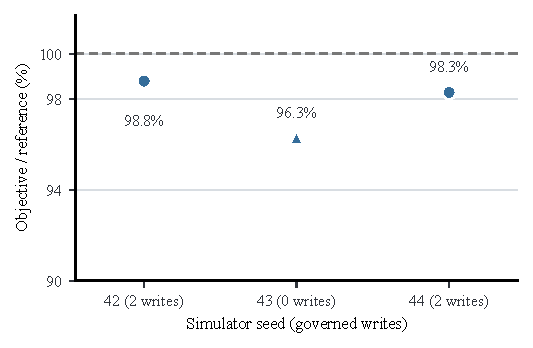
\includegraphics[width=0.96\columnwidth]{resources/fig-objective-ratios-current-run.pdf}
\caption{The three fixed-seed runner-defined end-score ratios ($J_{end}/J^*$)
were 96.3\%--98.8\% of the simulator's offline objective reference. Here
$J_{end}$ is the mean of the last two valid scores, or the sole valid score
when a case stops earlier; $J_{last}$ is the final individual trajectory
score. The dashed line marks 100\%; seed 43 stopped before any update.}
\label{fig:objective-ratios}
\end{figure}

\subsection{Scripted BOPET Integration Trace}
\label{sec:eval-bopet}
A separate task block in the same pipeline execution recorded three setpoint
writes to three distinct controls on a biaxially oriented polyethylene
terephthalate (BOPET) simulator scene. The thickness observations were
28.05, 27.98, 27.98, and $24.84\,\mu\mathrm{m}$, with the final reading inside
the configured $25.0\pm0.7\,\mu\mathrm{m}$ band. This trace demonstrates that the
configured scene and write path produced an in-band simulator observation;
it does not establish that the writes caused the endpoint or that an
optimization was completed. The task-board task reached COMPLETED, while its
associated parameter-change/optimization record remained open and unjudged;
the BOPET phase also contained the single semantic-card warning.
Fig.~\ref{fig:bopet-trace} shows this task separately from the fixed-seed
objective cases.

\begin{figure}[!t]
\centering
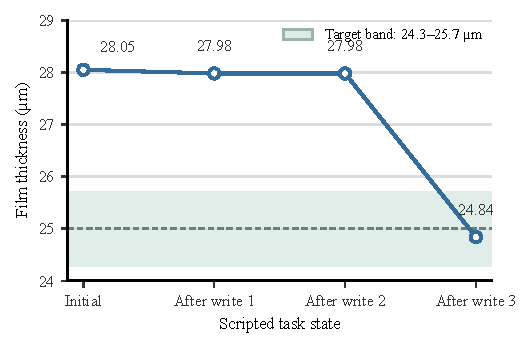
\includegraphics[width=0.96\columnwidth]{resources/fig-bopet-integration-trace.pdf}
\caption{One scripted BOPET task recorded an in-band terminal thickness of
 $24.84\,\mu\mathrm{m}$ after three writes. The shaded area marks the configured
$24.3$--$25.7\,\mu\mathrm{m}$ target band. The task-board task completed; its
associated parameter-change/optimization record remained open and unjudged.}
\label{fig:bopet-trace}
\end{figure}

\subsection{Evidence Boundary}
The run supports a bounded claim that the configured simulator paths connected
five protocol endpoints to data acquisition and that the tested negative
probes were rejected by the configured write guards. The objective ratios and BOPET
trace are separate simulator observations within this run. Because the
language-model loop was disabled, the platform and simulator were already
running, no conventional controller baseline was used, and no physical
equipment was involved, the evidence does not establish autonomous agent
behavior, comparative control benefit, cold-start commissioning, independent
repeatability, or field performance. Post-run hashes verify the delivered
evidence files, not the runtime configuration at execution time.

\section{Discussion}
\label{sec:discussion}
\subsection{Interpretation}
The integrated execution shows that configured scene mappings and a shared
operation boundary can be exercised together in a deterministic simulator.
Five protocol endpoints returned acquisition samples, and the tested negative
probes were rejected by the configured write guards. A second scene configuration
also exercised the guard path within the same pipeline invocation. These
observations support integration across the tested configurations; they do
not establish that arbitrary industrial scenes can be connected without
commissioning or route-specific configuration.

The seeded objective cases and BOPET task are separate observations, although
both were recorded by the same pipeline execution. The objective cases
compare selected simulator scores with an offline reference. The BOPET trace
records one scripted sequence of setpoint changes and a terminal thickness
inside the configured band; the task board marked the task COMPLETED, while
the associated parameter-change/optimization record remained open and unjudged.
Neither result provides a matched controller comparison, and the BOPET trace
does not isolate the effect of each write. The architecture and these
observations therefore describe a governed integration path, not autonomous
agent control or demonstrated process improvement.

The design complements work that grounds industrial actions in digital-twin
state, asset models, process diagrams, or supervisory checks
\cite{gehrmann2020dtiacs,graul2026aas,schall2026safe}. Its distinguishing
emphasis is the configuration boundary between task or harness execution,
scene-specific signal and driver mappings, and a shared device-operation path.
The current evaluation tests selected links across this boundary. It does not
measure whether configuration reduces integration time, maintenance effort,
or operational risk; those claims require matched deployments and workload
measurements.

\subsection{Scope and Limitations}
The evaluation used deterministic tool calls and local simulators. The
language-model loop was disabled, and the platform and simulator were already
running with shared data present. The run therefore does not test autonomous
LLM behavior or cold-start commissioning. Its three fixed-seed cases are
subcases of one pipeline execution, not independent system repetitions. One
seed stopped inside the configured region before updating, so the objective
results do not establish iterative convergence across initial conditions.

No conventional controller baseline, approval-on/off ablation, or physical
equipment was included. The negative probes support only the tested software
guard behavior; they do not measure human-approval effectiveness or establish
plant safety. The BOPET task's unjudged parameter-change/optimization record
and semantic-card warning further limit interpretation of its in-band endpoint.
Protocol latency summaries are retained in Supplementary File~S6 as
diagnostics only because the run did not
preserve event-level timings or complete denominators. The delivery manifest
was created after execution and does not establish a runtime-frozen
configuration.

The results therefore support an integrated simulator demonstration. Assessing
effectiveness requires independent system runs with a frozen configuration,
complete request-to-readback records, and matched controller and
approval-policy conditions, followed by hardware-in-the-loop evaluation.

\section{Conclusion}
\label{sec:conclusion}
This paper presents a configuration-driven architecture that connects
industrial task execution to scene-specific signals and protocol drivers
through a shared, governed operation interface. In one deterministic
simulator pipeline run, 76 of 77 checks passed, five protocol endpoints
returned 54 samples, and all 24 negative probes on four writable paths were
rejected by the configured write guards. An in-run second-scene check rejected 9 of
9 additional probes and returned 51 acquisition samples. The seeded objective
cases and the separate BOPET task provide bounded simulator observations; one
seed performed no update, and the BOPET task-board task completed while its
associated parameter-change/optimization record remained open and unjudged.
The evidence supports configured multi-protocol integration and selected guard
behavior. It does not establish
autonomous-agent performance, comparative control benefit, independent
repeatability, or physical-plant performance.

\noindent\textbf{Data Availability:} Supplementary File~S6 and its evidence
archive contain selected records, source data, and figures from the integrated
run. The archive includes delivery-time checksums, not runtime signatures for
the original execution. No physical-plant data are included.


\balance
\bibliographystyle{IEEEtran}
% Keep IEEEtran's default bibliography size and leading.
\bibliography{resources/refs}

\end{document}
